\section{Network}

The CLAS12 network is shown in Fig.~\ref{fig:network_diagram}. Its main component is an Arista router that serves as the backbone for the entire system. The set of main DAQ servers is connected directly to the router by 40~Gbit links. Some front-end components with particularly high data rates are connected directly to the router by 10~Gbit links. Most of the front-end conponents, as well as the workstations are connected to the network switches using 1~Gbit links, while those switches are connected to the router by 10~Gbit links. Two 40~Gbit uplinks connect the entire system to the JLab Computer Center.

Most of the 1~Gbit links use copper wiring, while the 10~Gbit and 40~Gbit links use optic fibers, with the exception of short range server links where 40~Gbit wires are used.

The CLAS12 network shows adequate performance and a high level of reliability. With the projected CLAS12 data rates, it can be used ``as is'' for the foreseeable future.

\begin{figure}[hbt]
	\centering
	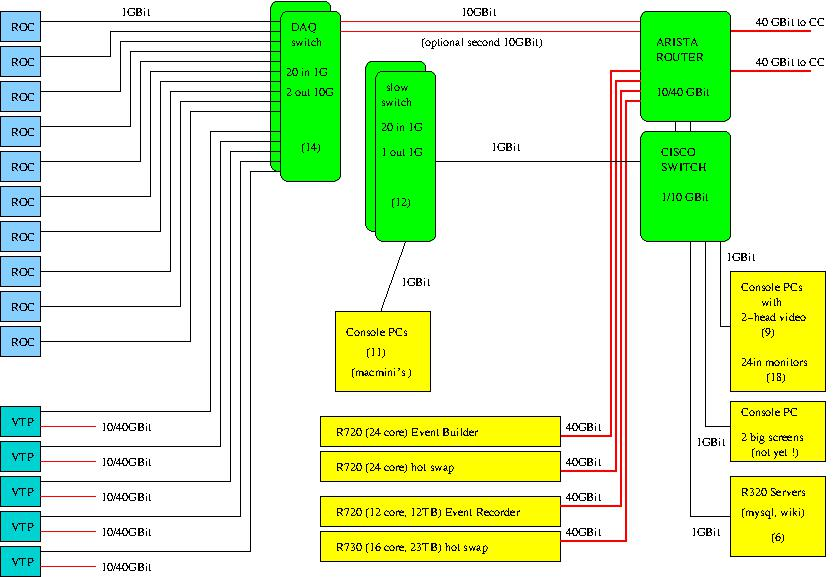
\includegraphics[width=1.0\columnwidth,keepaspectratio]{img/CLAS12_NET_1.jpg}
	\caption{CLAS12 DAQ Network Diagram}
	\label{fig:network_diagram}
\end{figure}
